\documentclass{scrartcl}

\usepackage{hyperref}
\usepackage{graphicx}

\begin{document}

\title{Gradr: Scalable Automatic Grading for Everyone}
\subtitle{System Overview, Load Testing, and Experience Report}
\author{Kyle Dewey, Jared Roesch, and Daniel Spokoyny}
\date{December 15, 2014}

\maketitle

\section{Introduction}
Gradr is a cloud-based system for automatically building, testing, and grading student solutions to class assignments.
The ultimate end goal of Gradr is to be used in MOOC-like settings, where it acts as a student submission system, an automated feedback generator, and an automated grader.

The goals of Gradr bring up a number of technical challenges relating to scalability.
Not only do the number of submissions become large in this setting, erratic usage patterns are a problem (e.g., many submissions just before a deadline).
For this reason, Gradr must be designed in a way which is not only scalable (for the overall load), but elastic --- we should be able to dynamically add and remove system resources as needed.

\section{System Overview}
Gradr is implemented as a distributed system with multiple components, which allows for concerns to be separated out and for horizontal scaling to be inserted at key points.
Where possible, we have used components from elsewhere which satisfy our needs.
A description of the different components in Gradr follows:

\begin{description}
  \item[GitHub~\cite{github}] \hfill \\
    A publicly-available hosting service for code repositories, focused around the \texttt{git}~\cite{git} revision control system.
    GitHub stores student solutions, lifting the burden of code storage off of Gradr.
    GitHub also informs the rest of the Gradr system whenever code is submitted (via a typical \texttt{push}), triggering downstream building to occur.

  \item[Postgres~\cite{postgres}] \hfill \\
    A popular relational database engine, which serves to store persistent information.
    Postgres also facilitates communication between different components of Gradr, as it stores globally synchronized state.

  \item[Notification Listener] \hfill \\
    A custom component which listens for \texttt{push} notifications from GitHub via a webhook~\cite{github_webhook}.
    Whenever a student performs a \texttt{push}, GitHub performs a standard POST request to this service, providing:
    \begin{itemize}
      \item The unique GitHub username of the student performing the \texttt{push} (which is ultimately mapped back to a unique username in Gradr)
      \item The name of the repository the student \texttt{push}ed to (which is ultimately mapped back to a unique assignment identifier in Gradr)
      \item The branch on which the \texttt{push} occurred
    \end{itemize}
    The above information is put into the Postgres database, and is marked as pending for downstream processing.

  \item[Worker] \hfill \\
    A custom component which regularly polls the Postgres database, looking for student submissions which are marked as pending.
    The worker will first select a pending entry, and mark it as being processed.
    The worker will then download the submission from GitHub, compile it, run tests, and put the test results pack into the Postgres database, finally marking the entry as complete.
    Crucial to Gradr's design is the fact that there can exist any number of worker components at any time.

  \item[Frontend] \hfill \\
    A custom web application which students and instructors can use to view feedback on their submissions, which was derived from workers.
    Much like workers, there can exist multiple frontend components at any time.
\end{description}

A graphical representation of these components, along with the data flow between them, can be seen in Figure~\ref{fig:system_overview}.

\begin{figure}[here]
  \begin{center}
    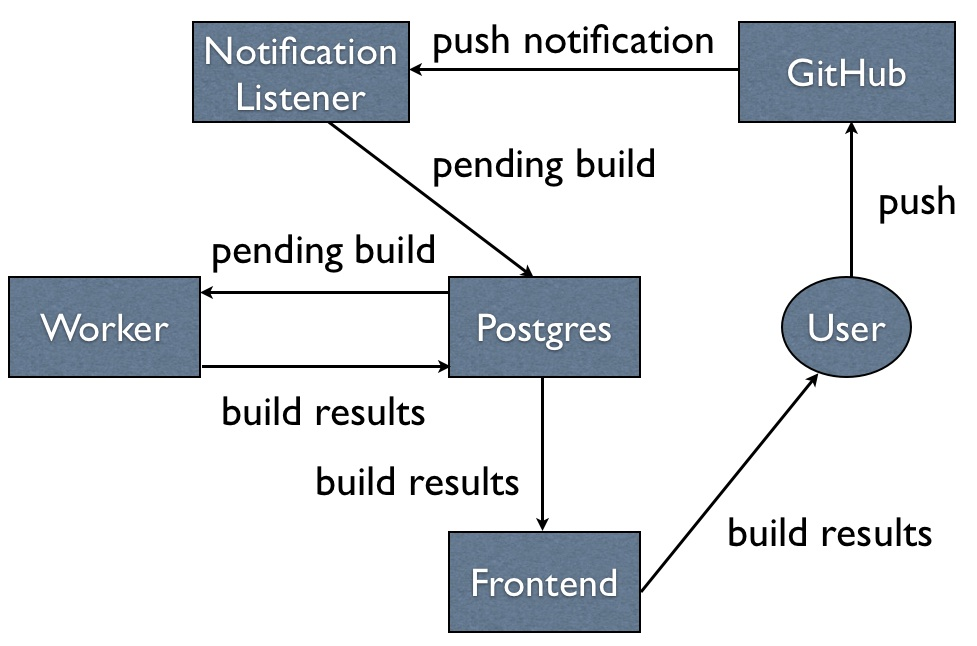
\includegraphics[scale=0.45]{non_graph_images/system_overview.jpg}
  \end{center}
  \caption{Diagram of overall Gradr architecture, along with data flow between components and the user}
  \label{fig:system_overview}
\end{figure}

\section{Load Testing}
\subsection{Critical Paths}
With respect to how Gradr is intended to be used, we identify three critical paths:

\begin{itemize}
  \item The process of polling pending builds from the database and putting results into the database
  \item The process of putting a pending build into the database from a GitHub \texttt{push} notification
  \item Users viewing build results on the frontend
\end{itemize}

The rest of the report focuses on the first of these tasks, as it is expected to be the most executed part of the architecture.

\subsection{Experimental Setup}
For all experimenents, we used RDS~\cite{rds} with a single \texttt{db.ts.small} instance.
As we focus only on builds, the number of notification listeners and frontend systems was kept constant at one.

Submitted code was carefully controlled, and kept uniform for the duration of individual experiments.
The actual submitted code can be found at \url{https://github.com/kyledewey/test-gradr}.
Two student submissions were used, described below:
\begin{description}
  \item[sleephalf] \hfill \\
    Under the \texttt{sleephalf} branch, the code when run will sleep for a half of a second, and then print out some fake test results.

  \item[sleep3] \hfill \\
    Under the \texttt{sleep3} branch, the code when run will sleep for a three seconds, and then print out some fake test results.
\end{description}

The reason why both submissions simply sleep as opposed to doing a real code build and test cycle is because this cuts out large amount of variability between individual instances.
We can know for sure that the build should take a precise, fixed amount of time under all circumstances.
This allows us to focus in on communication overhead within the system and other related issues.
While this unit time property is unrealistic, in practice, issues pertaining to CPU or IO-intensive builds could be simply adjusted by using bigger instance types, and these are not issues fundamental to Gradr itself.

Workers were distributed in five different ways, described below:
\begin{description}
  \item[One Small] \hfill \\
    A single worker process runs on a single \texttt{t2.small} EC2~\cite{ec2} instance.

  \item[Two Small] \hfill \\
    Each of two \texttt{t2.small} EC2 instances run a single worker process.

  \item[Four Small] \hfill \\
    Each of four \texttt{t2.small} EC2 instances run a single worker process.

  \item[One Large] \hfill \\
    Two worker processes run on a single \texttt{m3.large} EC2 instance.

  \item[Two Large] \hfill \\
    Each of two \texttt{m3.large} EC2 instances run two worker processes.
\end{description}

For all experiments, we sent 100 push notifications of whichever chosen repository and branch to the notification listener, initially with no running workers.
Once all notifications were sent, workers were started in parallel in the formation according to whichever AWS configuration was chosen.
While experiments are running, we measure the number of pending builds (queue length) over time.
Once an experiment finishes, we determine the average amount of time each build took, starting from the point where a build was selected for processing and ending with the time the results were posted.

The goal with measuring the queue length over time is to identify any anomalies in communication.
We would expect in all cases a straight line, and any other shape would indicate issues like contention.

The goal with measuring the average time of each build is to determine the overall overhead of the system itself.
Since the time each build takes is known in advance, we know that any additional time is purely overhead of our system.

The goal with varying the instance configuration is to identify any sort of unseen computational and network bottlenecks, along with measuring scalability of the system.
If the worker process is CPU-intensive independent of the actual student code, then this would reveal itself as bigger instance types performing better than smaller instance types.
Additionally, in a perfectly scalable environment we would expect to see that twice as many worker threads can clear a queue of pending builds in half the time, and so on.
This would not be true of a high-contension situation, and would be strong cause to optimize.

\subsection{Results and Discussion}
\section{Possible Improvements}
\subsection{Frontend}
Put it behind a load balancer.

TODO: actually describe this.
\subsection{Backend}
\subsubsection{Notification Listener}
Make multithreaded, put behind a load balancer.

TODO: actually describe this.
\subsubsection{Worker}
If a worker fails, it can leave the system in an inconsistent state, where a submission is marked as submitted but is never built.
This can be addressed by using a fault-tolerant queue like SQS~\cite{sqs} for communication between the notification listener and workers.

TODO: actually describe this.
\subsubsection{Postgres}
Read replications.

TODO: actually describe this.

\subsubsection{Auxilliary Storage for Results}
Results can be huge, and are stored in Postgres right now for simplicity.
These could be put into an auxilliary, eventually consistent data storage if downloading results from Postgres becomes a burden.

TODO: actually describe this.

\section{On the Usage of the Rust Programming Language}
The entire backend is implemented in the Rust programming language~\cite{rust}.

\subsection{Advantages and Challenges}
\subsection{Database Operations}

\bibliography{bibtex}{}
\bibliographystyle{plain}

\end{document}
